\documentclass[letterpaper, 12 pt, conference]{ieeeconf} 
\IEEEoverridecommandlockouts                           
\overrideIEEEmargins

\usepackage{graphicx}
\usepackage{verbatim}
\graphicspath{ {./images/} }

\title{\LARGE \bf
Analog Synthesizer with Digital Control
}

\author{Aros Aziz$^{1}$, Jay Heiland$^{2}$, and Michelle Simmons$^{3}$ \\ https://jayheiland.github.io/CE\_Senior\_Project% <-this % stops a space
\thanks{$^{123}$A. Aziz (arosaziz96@gmail.com), J. Heiland (jay.heiland@gmail.com), and M. Simmons (michelle.simmons@utah.edu) are seniors in Computer Engineering at the University of Utah in Salt Lake City.}%
}

\begin{document}
\maketitle
\thispagestyle{empty}
\pagestyle{empty}

%%%%%%%%%%%%%%%%%%%%%%%%%%%%%%%%%%%%%%%%%%%%%%%%%%%%%%%%%%%%%%%%%%%%%%%%%%%%%%%%
\begin{abstract}
The goal of this senior project was to take the best parts of both digital and analog synths and combine them into a working, scalable prototype for an analog synth with digital control. The core components of this project consist of a software application, synthesizer modules, and the software and hardware interfaces between them. On Demo Day we were able to show off the most important and core parts of our project, which could be scaled to a much larger product. 

\end{abstract}


%%%%%%%%%%%%%%%%%%%%%%%%%%%%%%%%%%%%%%%%%%%%%%%%%%%%%%%%%%%%%%%%%%%%%%%%%%%%%%%%
\section{INTRODUCTION}
Synthesizers are musical instruments that have been popular with musicians and producers for decades. Synths see ubiquitous use in the popular music of today, and it is safe to assume that many of the artists that use them are using their digital variety; that is, using digitally simulated audio circuits on a computer via services like Ableton Live or Serum. These digital modules are often much cheaper than their older, analog counterparts. In addition, they give users the ability to save the settings of their favorite sounds, allowing them to revisit previous patches with the click of a button. Despite digital synths' advantages in cost and convenience, many artists are now returning to analog synths for their (perceived) better sound quality \cite{MAKE}. Unfortunately, what these artists gain in quality they lose in convenience. 

Our senior project takes the best of both the digital and the analog synths; it marries the superior sound production of the analog synth modules with the convenience of the digital synth. We designed analog circuits to produce and modify audio signals, where each circuit has its variable resistances controllable by a computer. In addition to reading and setting the values of the variable resistances (potentiometers), our desktop application can also save settings and load them back on at a later time, providing the artist with the same level of convenience as a traditional digital synth.

Our project comprises of three major parts: our software application, our modules, and the software and hardware that interfaces between them. Our MIDI keyboard serves as an important peripheral that makes the demo of our project interactive and exciting. By the beginning of fall semester, we had decided not to pursue our stretch goal of implementing an automated switch matrix between the modules, as none of us believed we would have the time, skill, or interest to work with the mechanical hardware.

We have three total modules: a voltage controlled oscillator (VCO), a high-pass voltage controlled filter (high-pass VCF), and a low-pass voltage controlled filter (low-pass VCF). By the time of the demo on Demo Day, only our VCO could be demoed. Both our HP VCF and our LP VCF had been working the previous afternoon; unfortunately, we used the last of some of our expensive parts in the attempt to mount the VCFs onto strip-boards. After Demo Day, we decided as a team that we are pleased with our final demo, and not to pay for new parts and shipping at great expense in order to fix our VCFs.

Our software application provides an easy and attractive way to control the synth, with all the technical details hidden completely behind-the-scenes. Using the desktop application, users can change potentiometer values on each individual module, save the values of each module, and load old configurations. The application also always displays current potentiometer values, even if they are changed physically (via rotary encoder) rather than digitally. 
The integration between our desktop application and our modules consists of embedded C code, which is robust and scalable. The embedded code allows a computer to read from and write to the values of the potentiometers on the digipot chips. It also allows rotary encoders to change the values of those potentiometers. These two capabilities are what allow both the physical and digital control of the analog synth’s sound. 

\section{TECHNICAL DESIGN}
As mentioned in the introduction, our project is made up of three major parts: the software application, the modules, and the software and hardware interfaces between them. The following sections will go into detail of each of these parts and explain how they were designed and some of the challenges that went with them.

\subsection{Synth Modules}

We have three modules: a VCO, a high-pass VCF, and a low-pass VCF. Voltage control is an important concept in modular synthesis, and we utilized it in all three of our modules. Each module has a control voltage (CV) input that modulates its output. In the VCO, the input control voltage dictates the frequency of the VCO's output. In this case, the CV is discrete; each discrete voltage corresponds to a distinct pitch. This CV was supplied by the MIDI controller keyboard at our demo; the CV input to the VCO is what made the synth playable like a piano. In the VCFs, the CV was continuous. We chose to simulate a low-frequency oscillator (LFO) as the CV input to the VCFs, and we did so by using the function generator to supply a 1 V peak-to-peak sine wave at a frequency of 4 Hz. The LFO/VCF combination is a common one in musical synthesis. The CV causes the output signal of the VCF to audibly pulse in time with the LFO. 

The design of these modules turned out not only to be technically challenging, but also expensive. We breadboarded and tested each module individually before we augmented them with digipots and rotary encoders. 

\begin{enumerate}
    \item VCO
    
    Our VCO is the music generator of our synth. It recieves CV input and produces a variable-frequency audio signal as output. Its most important component is the CEM3340, a VCO chip. The module has as its outputs both a triangle wave and a sawtooth wave; the user may choose which waveform to use by choosing the corresponding audio jack, labeled clearly on the PCB for the VCO.
    
    \begin{figure}[ht]
    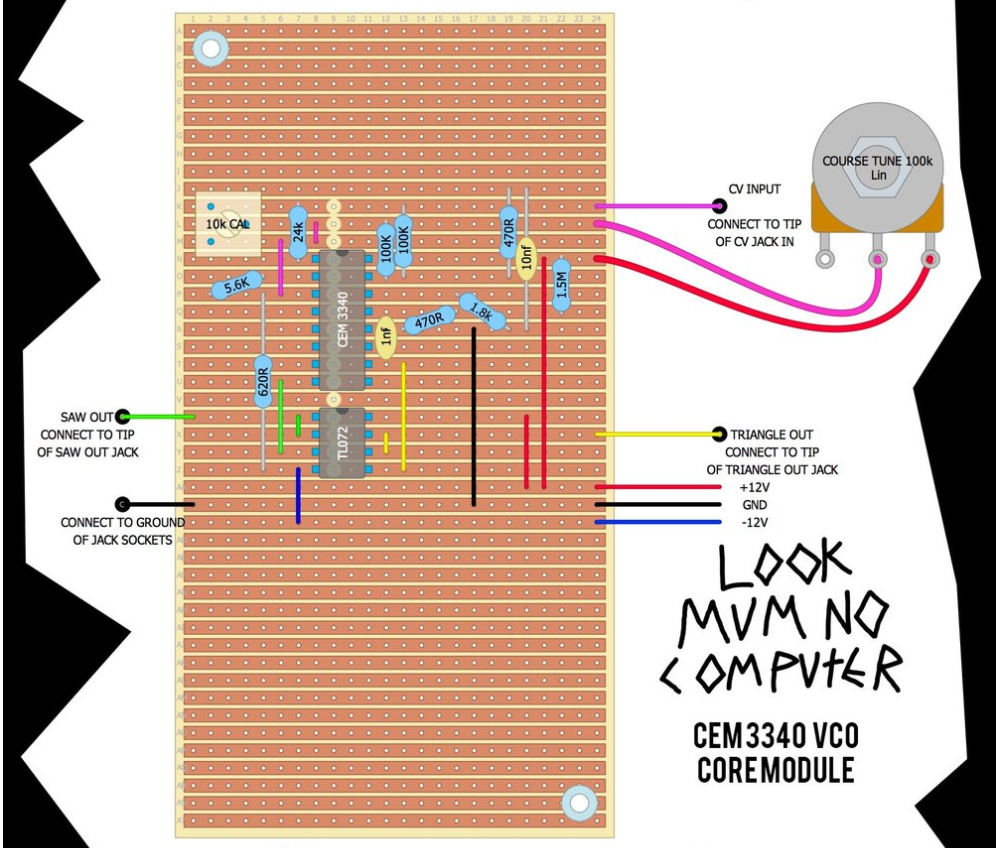
\includegraphics[width=8cm]{VCO}
    \centering
    \caption{Original schematic for VCO \cite{VCO}}
    \label{vcofig}
    \end{figure}
    
    The Coarse Tune 100 Kohm potentiometer in the schematic, which we later replaced with a digipot, changes the pitch of the output. So while you play Mary Had a Little Lamb on the keyboard, if you change the value of that potentiometer, your entire song may shift to be two octaves higher, but it will still be the original song.
    
    Part of our original hardware was a custom PCB designed using Eagle and ordered through OshPark. Fig. \ref{schfig} shows the PCB schematic for the VCO.
    
    \begin{figure}[ht]
    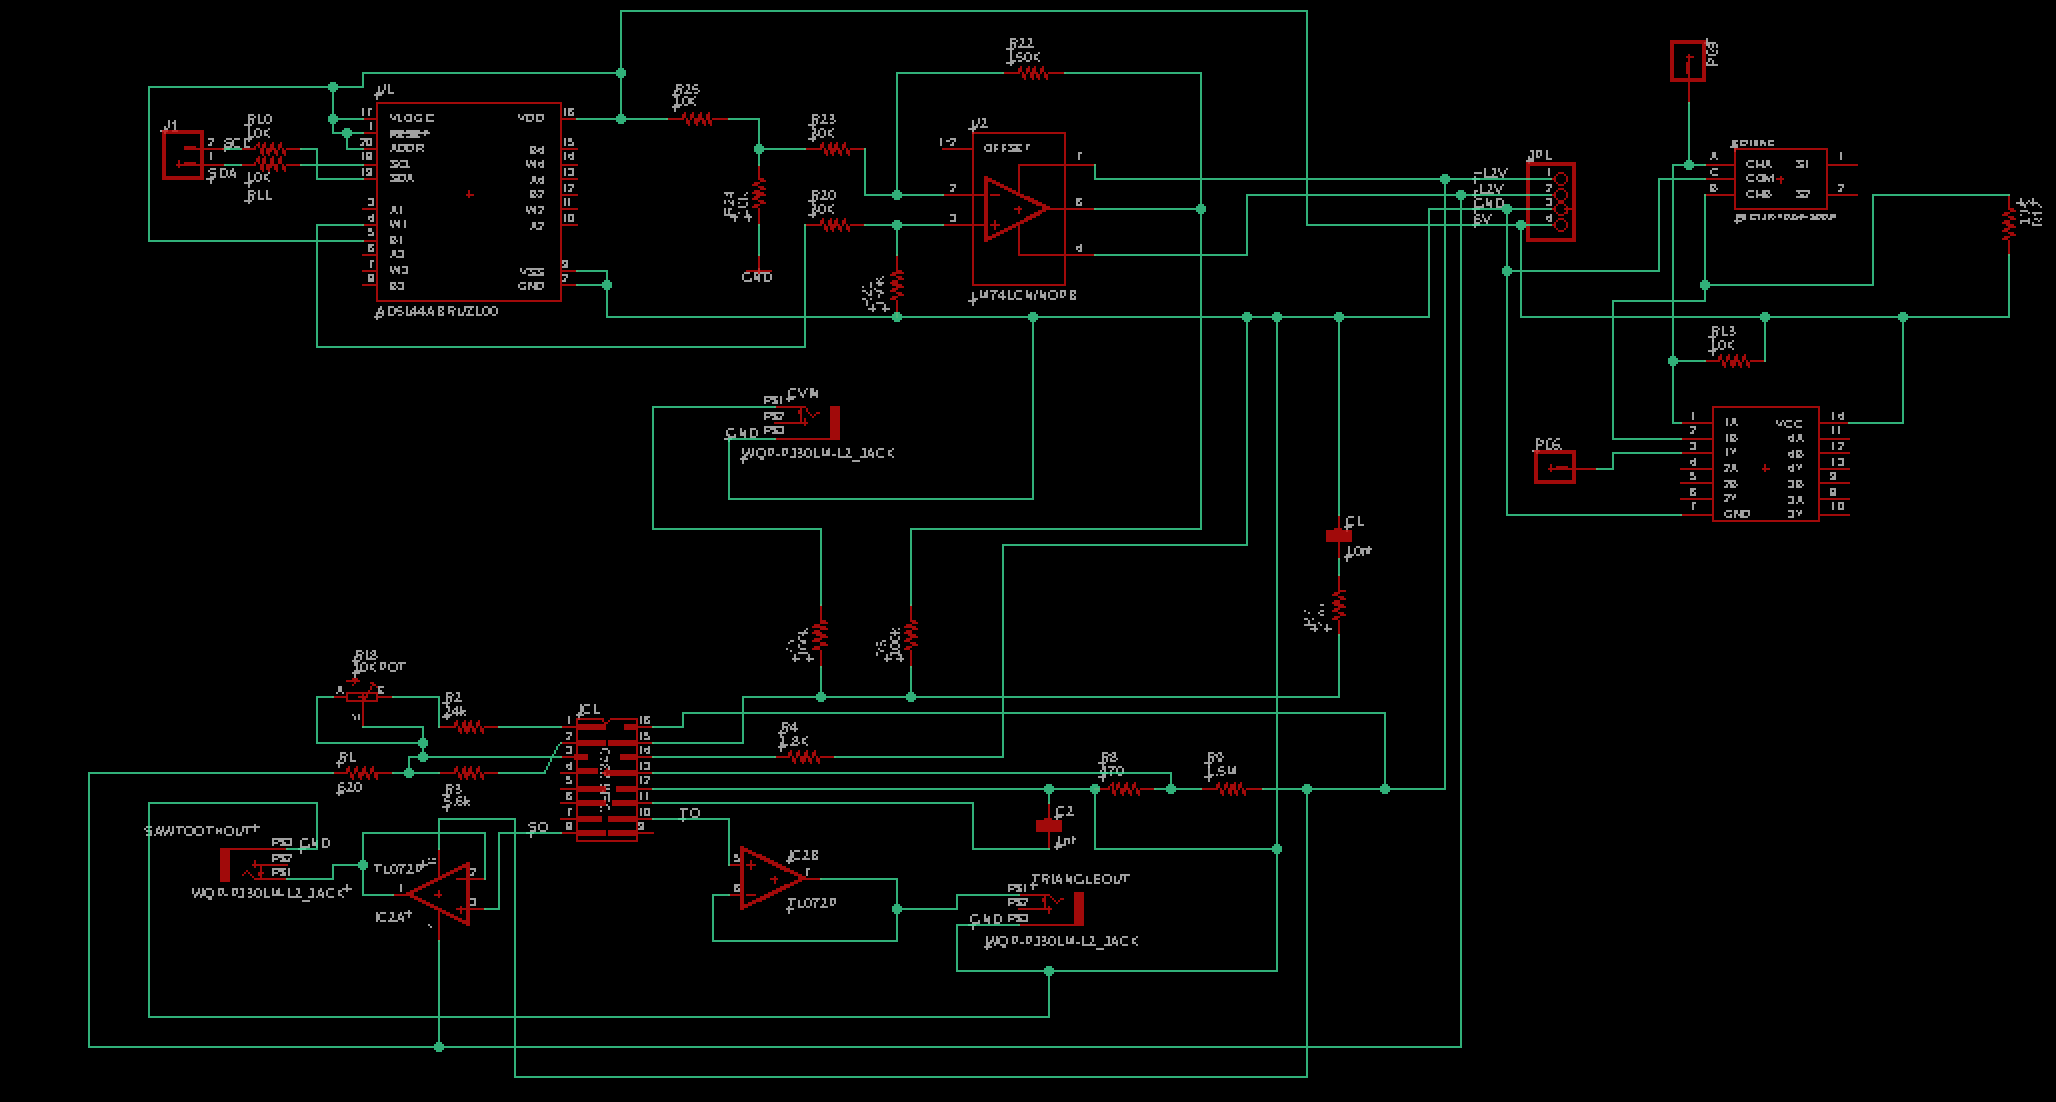
\includegraphics[width=8cm]{images/pcbschem.png}
    \centering
    \caption{PCB schematic of the VCO}
    \label{schfig}
    \end{figure}

    This schematic includes custom footprints that we either created or found on the web and modified in order to meet the specifications of our breadboarded prototype.

    In addition to creating the schematic, the footprints had to be placed in positions that were optimal for the wiring between components. Many attempts were made to find the optimal solution and eventually one was found to be the best positioning for all the parts. In addition to placement design, we needed drilled holes on the four corners of the custom board so that we could screw it through an acrylic attached to the Eurorack case at the end for Demo Day purposes. Fig. \ref{pcbfig} shows an image of the PCB design of the finalized custom PCB.
    
    \begin{figure}[ht]
    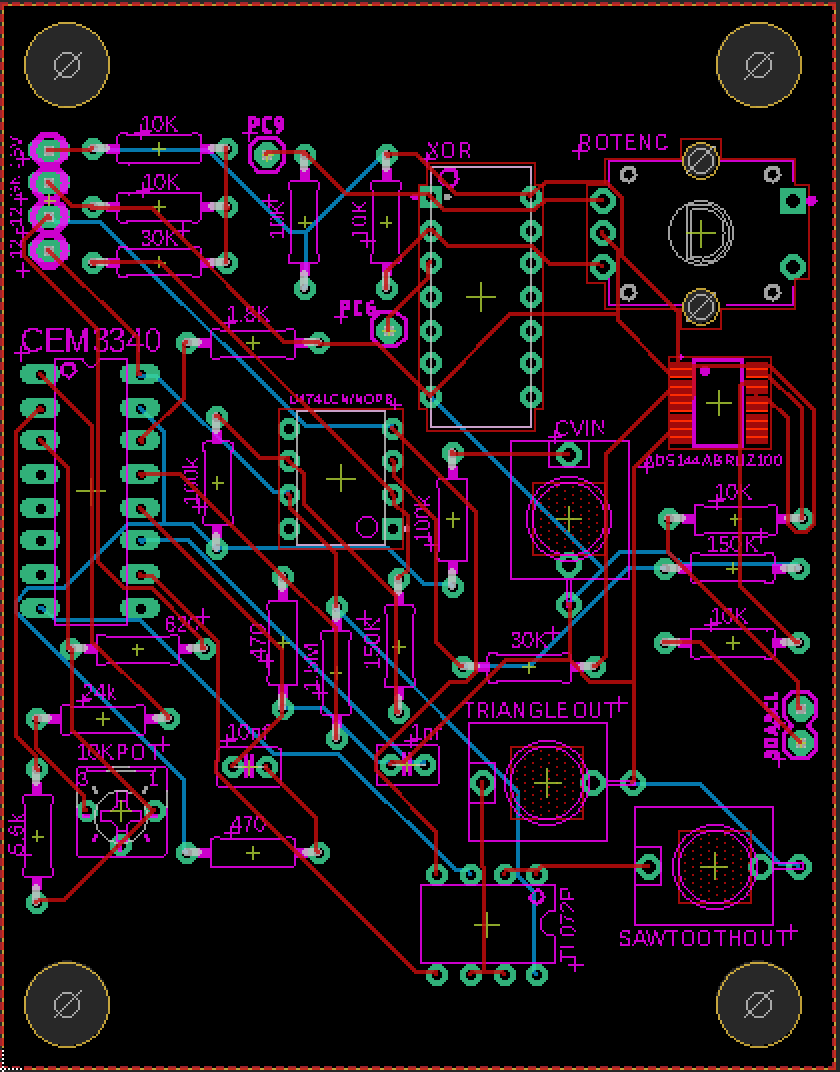
\includegraphics[width=8cm]{images/pcbdesign.png}
    \centering
    \caption{PCB design of the VCO}
    \label{pcbfig}
    \end{figure} 
    
    For the sake of easy soldering, we made an effort to make sure that a majority of the components were through-hole. In the end, we were able to make sure every part going onto the board was through-hole except for one, which was the digital potentiometer.
    
    \item VCFs
    
    The VCFs each take two inputs: audio signal and CV. The audio signal could feasibly come from any source, but in our synth, it was most practical (and made for the best sound) to use the output from the VCO. The CV input came from the function generator's LFO. We determined early on in the semester that an LFO module would be too complicated for us to tackle, but with more time, we could build an LFO and easily integrate our digipot and rotary encoder to make it a fully functional module in our unique synth.
    
    The original schematics for the VCFs do not allow the user to control the cutoff frequency of the filters, so we added that feature. These changes are shown via the original and modified schematic of the low-pass VCF, in Fig. \ref{lpffig} and Fig. \ref{modlpffig}, respectively.
    
    \begin{figure}[ht]
    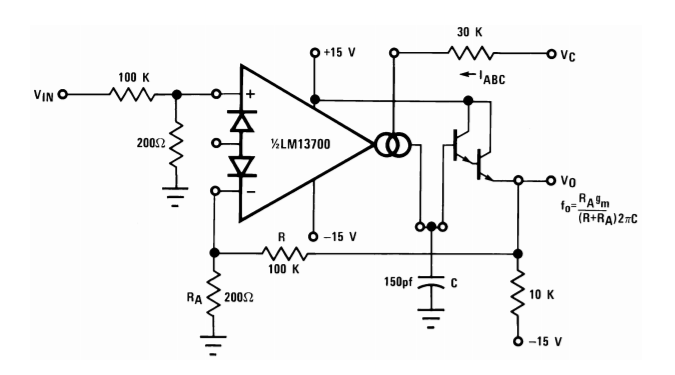
\includegraphics[width=10cm]{LPF}
    \centering
    \caption{Original schematic for Low-Pass VCF \cite{VCF}}
    \label{lpffig}
    \end{figure}
    
    Notice the lack of any potentiometers in Fig. \ref{lpffig} that would allow the user to change the cutoff frequency of the filter. Pay particular attention to the input labeled "Vc," as that is where our changes were made. Those changes are shown in Fig. \ref{modlpffig}.
    
    \begin{figure}[ht]
    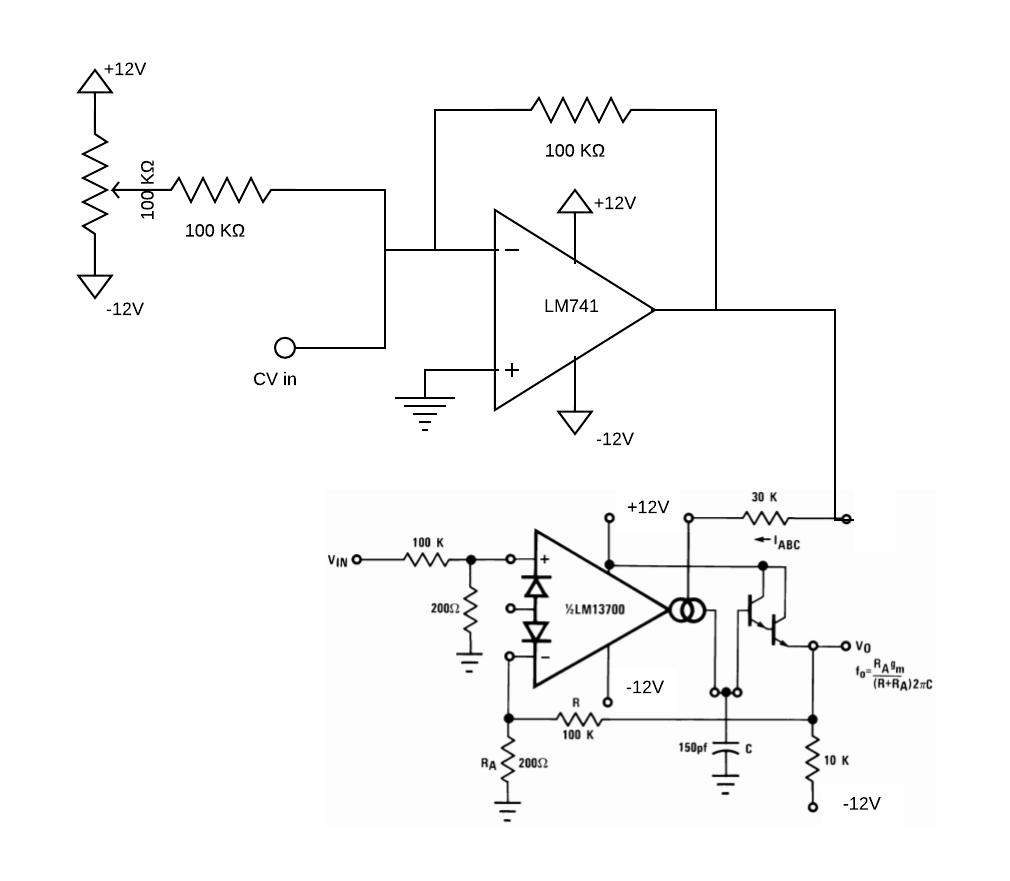
\includegraphics[width=10cm]{modlpf}
    \centering
    \caption{Modified schematic for Low-Pass VCF}
    \label{modlpffig}
    \end{figure}
    
    The value of the 100 Kohm potentiometer controls the cutoff frequency of the filter. This is the potentiometer that would later become a digipot. The CV input and the voltage that determines the cutoff frequency are summed together in a summing amplifier to produce the final voltage that the original VCF sees. 
    
    The summing amplifier and potentiometer were added in the exact same fashion to the high-pass VCF, shown in Fig. \ref{modhpffig}.
    
    \begin{figure}[ht]
    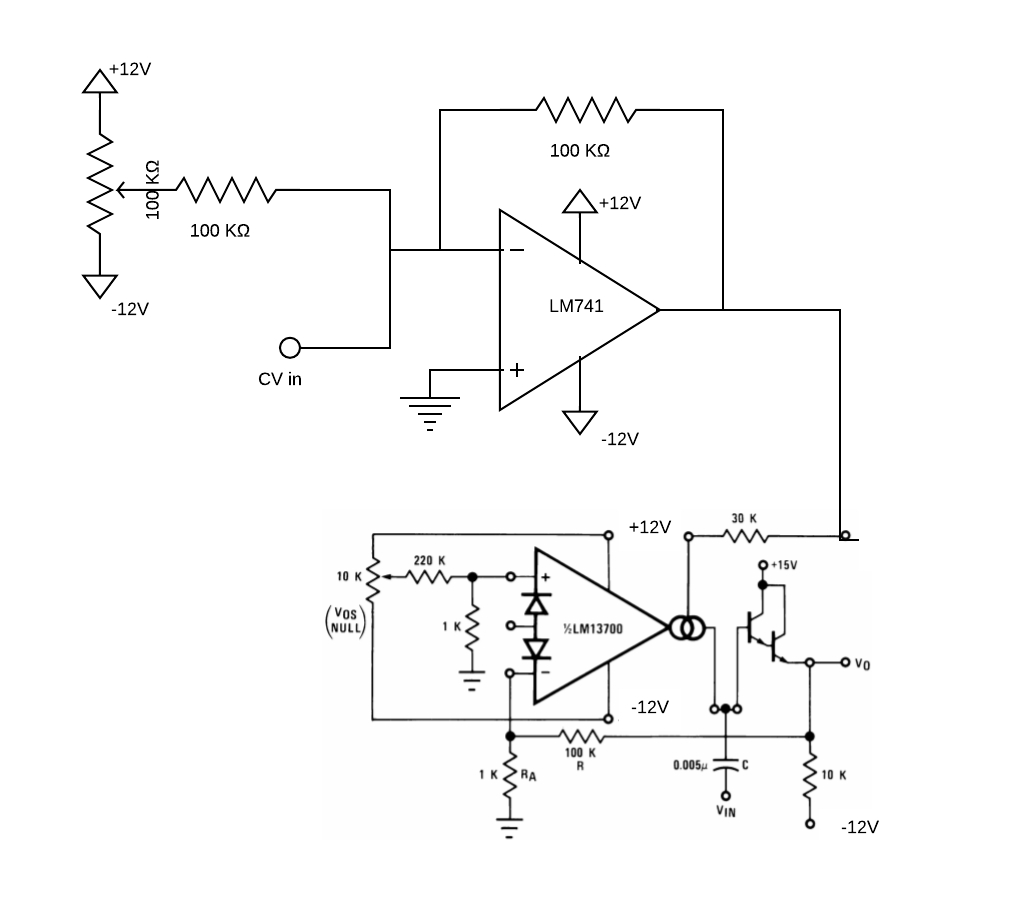
\includegraphics[width=10cm]{modhpf}
    \centering
    \caption{Modified schematic for High-Pass VCF \cite{VCF}}
    \label{modhpffig}
    \end{figure}
    
    Both of the VCFs were working with the digipots and rotary encoders the day before Demo Day. That evening, in an attempt to make the demo looking as polished as possible, we tried to solder the VCFs to strip-boards. Unfortunately, once the soldering was finished, the VCFs no longer functioned--most likely due to an undetected short-circuit. In our exhaustion and hurry, we fried the last of our remaining components needed for the VCFs.
    
\end{enumerate}


\subsection{Embedded Software}

We used the AD5144 digital potentiometers in all three of our modules. The VCO used one chip, and the two VCFs shared a second chip. In the VCO, the digipot controls the pitch register of the output signal. In the VCFs, each digpot controls the cutoff frequency of its fitler. The digital potentiometers communicate with the microcontroller via the I2C protocol. Each digipot has its own address so that the master (microcontroller) knows which slave (digipot) it is dealing with. To acheive two addresses, the first digipot chip has its address pin (pin 20) connected to +5V, and the second digipot chip has its address pin unconnected \cite{pot}. Each chip has four individual potentiometers. Each potentiometer has two terminals and a wiper--for instance, A1, W1, and B1 represent one individual potentiometer.

\begin{figure}[ht]
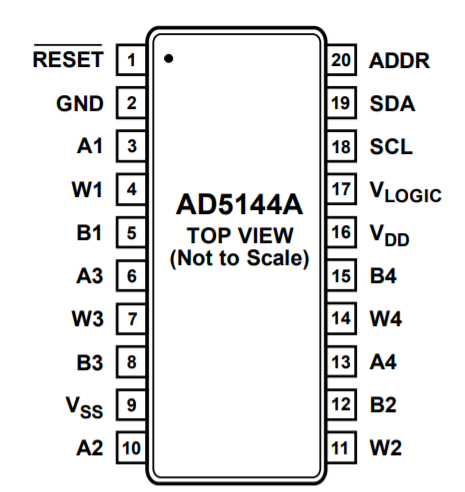
\includegraphics[width=6cm]{pot}
\centering
\caption{Pinout for the AD5144 digital potentiometer chip \cite{pot}}
\label{potpin}
\end{figure}

We used PEC12R rotary encoders, which use quadrature encoding \cite{rotenc}. The rotary encoders also communicate to the microcontroller through a series of interrupts.

We used the STM32F072 ARM Microcontroller to control and listen to the digipots and rotary encoders via I2C, and to communicate information to a computer via USART.

Our embedded code program allows the digipots and rotary encoders to communicate with the microcontroller via I2C, and it allows the microcontroller to communicate with the computer via USART. The flow of information is laid out in the diagram in Fig. \ref{i2cfig}, where the PCB represents the synth's modules. 

\begin{figure}[ht]
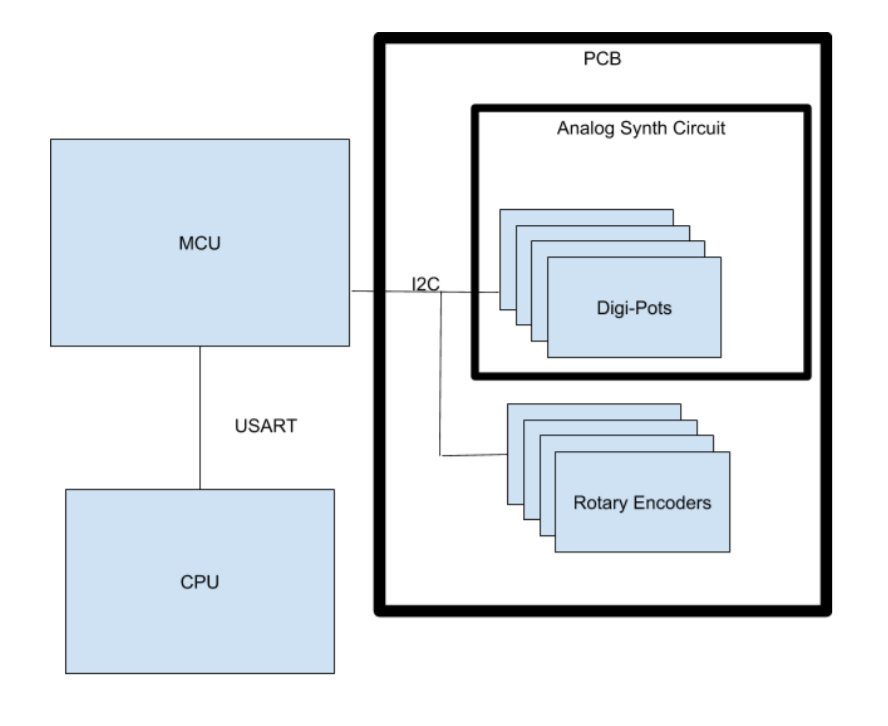
\includegraphics[width=9cm]{i2c}
\centering
\caption{Communication protocols between our circuits, the microcontroller, and the computer}
\label{i2cfig}
\end{figure}

The digipot communicates to the microcontroller through its SDA and SCL pins. The microcontroller can read the value of each potentiometer on each chip, or write to any individual potentiometer on either chip, on command. 

The first time we installed the digipot into our VCO, we fried the chip. The AD5144 can only endure a maximum voltage difference of 5V, and we had connected it to +12V and -12V, exposing it to a voltage difference of 24V. To limit its exposure, we designed an amplifier circuit that amplifies the 0 to 5V output of the digipot to the -12 to +12V voltage that the VCO expects. We used the LM741 amplifier to do this. 

Fig. \ref{digfig} shows the connection between the microcontroller and the digipot chip, as well as the amplifier circuit. 

\begin{figure}[ht]
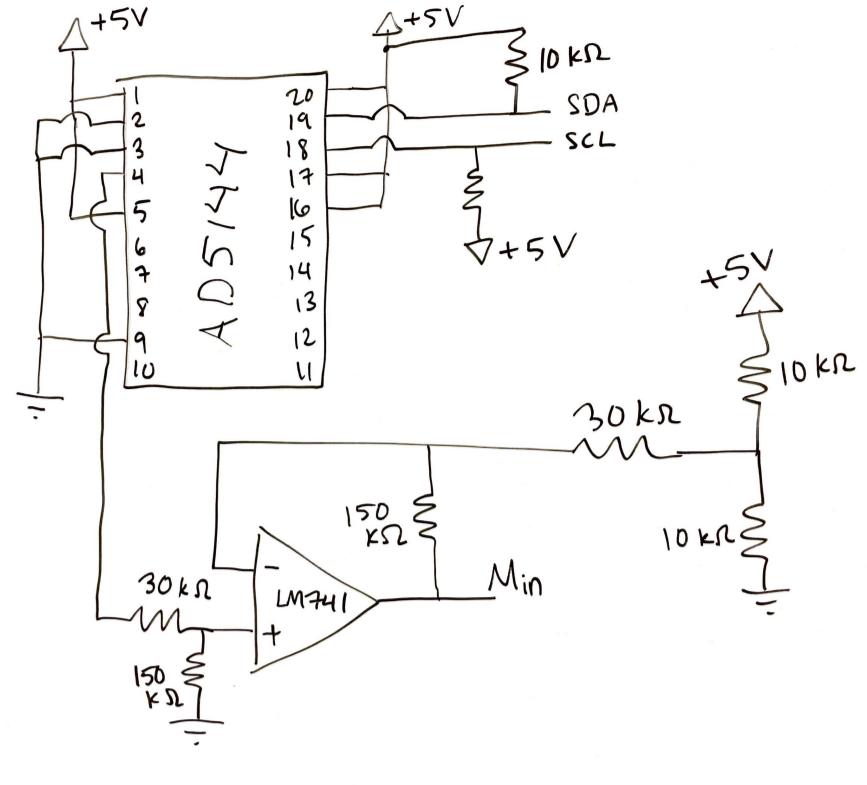
\includegraphics[width=9cm]{digipot}
\centering
\caption{Digital potentiometer chip's connections to module and microcontroller}
\label{digfig}
\end{figure}
The amplifier circuit connects to any given module at $M_{in}$. Only one potentiometer is shown wired to a module in the figure, for simplicity. In practice, though, all four potentiometers on the chip could be used in synth modules, each potentiometer with its own amplifier circuit.


The rotary encoder works slightly differently; it communicates to the microcontroller through interrupts. Observe Fig. \ref{rotencfig}. The two terminals of the rotary encoder are wired to a single XOR gate; whenever the knob of the rotary encoder is spun, that movement is reflected by a change in exactly one of those terminals. Thus, the output of the XOR gate will change every time the rotary encoder is spun. The output of the XOR gate is wired to the microcontroller (in Fig. \ref{rotencfig}, labled PC6) so that every time its value changes, an interrupt is triggered. When this interrupt occurs, the embedded code checks the value of one of the terminals (in Fig. \ref{rotencfig}, labeled PC9) to see whether the encoder was turned left or right. If left, the microcontroller sends the associated potentiometer a command to increase its value. If right, a command to decrease. 

\begin{figure}[ht]
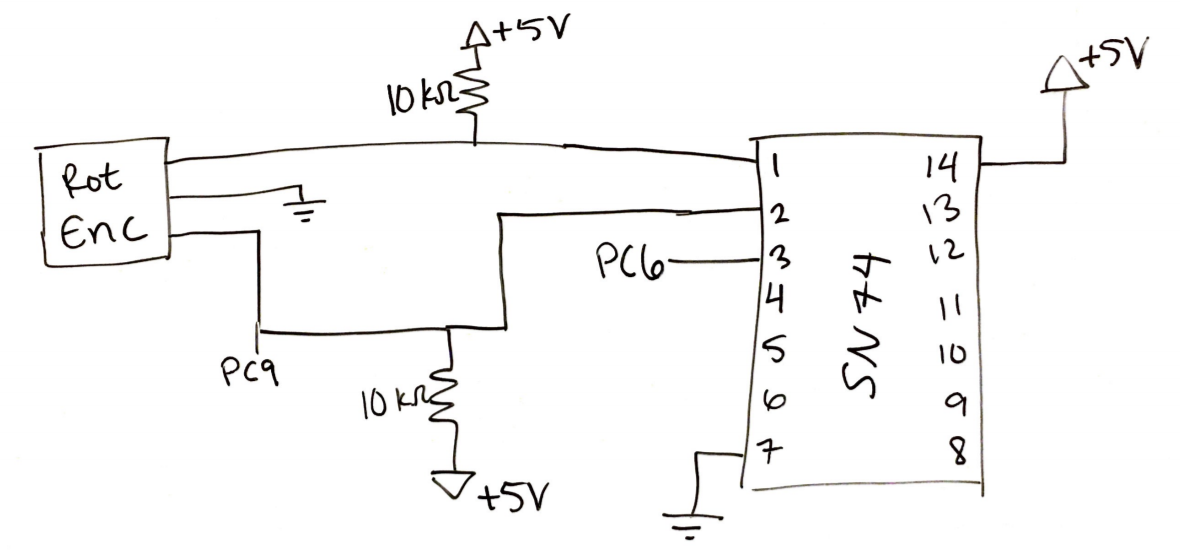
\includegraphics[width=9cm]{rotenc}
\centering
\caption{Rotary encoder and XOR gate, and their connections to the microcontroller}
\label{rotencfig}
\end{figure}

In order to replace an analog potentiometer with a digital one, simply remove the analog potentiometer entirely and reconnect its old connections to the digital potentiometer. Be careful: replace voltages above 5V with 5V, and voltages below 0V with ground, to ensure that the digipot never sees a voltage difference greater than 5V. The digipot and rotary encoder combination are an extremely scalable component of our project. They could easily be implemented in any synth module, without any further modifications. Time and cost were our only barriers from adding more modules to our synth; any additional modules would have been immediately ready to communicate with our desktop application.
    


\subsection{Desktop Application}

In addition to the embedded software, we created a supporting desktop GUI application in Python to fulfill the original software requirement. We called it "MySynth". As described in our project proposal, this desktop app allows the user to change the values of each module (just the VCO in our demo), save/load ".preset" files containing these values, and swap between loaded presets. The app relies on the pyserial Serial class for sending and receiving information from the STM32F072 microcontroller, and relies on the Kivy GUI application development library, including an official file dialog script \cite{pyserial} \cite{filechooser}.

\begin{figure}[ht]
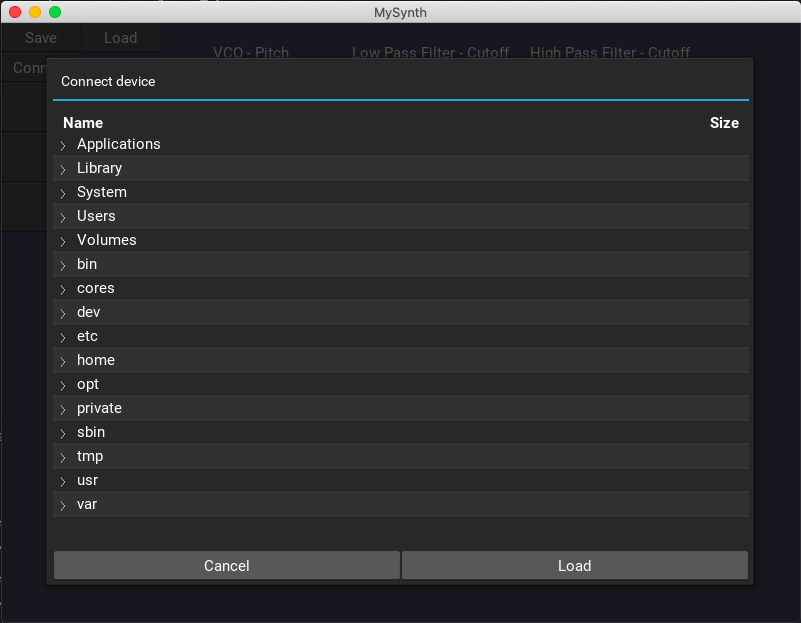
\includegraphics[width=9cm]{images/app_file_dialog.png}
\centering
\caption{File dialog in MySynth for connecting to an STM32F072 device}
\label{app_connect}
\end{figure}

Fig. \ref{app_connect} shows the file dialog used for connecting to the microcontroller. Once the user locates and clicks on the STM's port in this file dialog, the app creates a new Serial object to handle serial communication between the MySynth app and the microcontroller \cite{filechooser}.

\begin{figure}[ht]
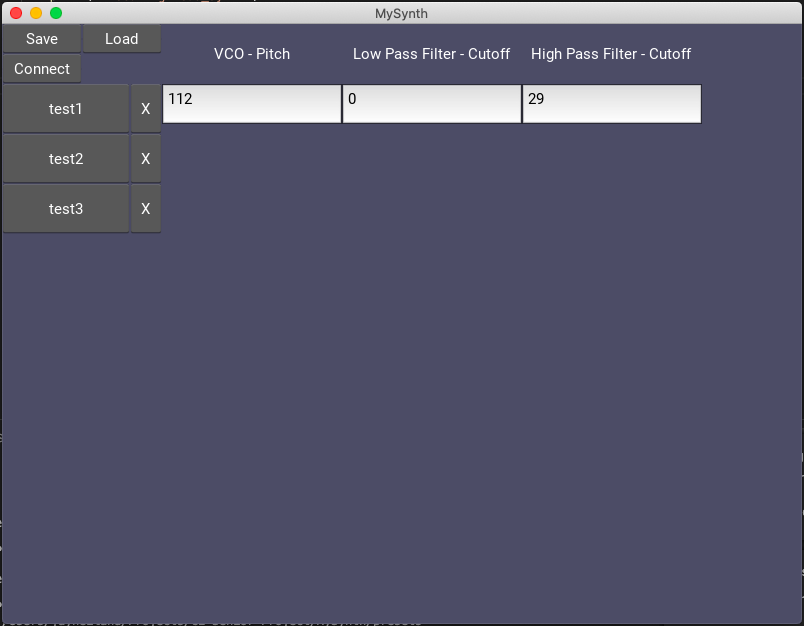
\includegraphics[width=9cm]{images/app_main.png}
\center
\caption{Default appearance of MySynth app, with presets loaded}
\label{app_default}
\end{figure}

Fig. \ref{app_default} shows how the app appears after the user has loaded a few presets. The user can click a preset button in the sidebar to load those values into the GUI, or close a loaded preset by clicking the associated "X" button. The app uses a separate thread to periodically read the current value of a module's digital potentiometers via the microcontroller. These values are then written to the GUI. This means that the user can tweak a module's value using its physical encoder knob and see that new value appear in the GUI. When the user clicks into a module's GUI text input, the "reading thread" pauses for a while, allowing them to enter new values. When the user clicks the "enter" key, those new values are written to the module's digipots via the microcontroller, and the reading thread resumes. In retrospect, we should have used one set of text display widgets that the reading thread updates with the current digipot values, and a different set of text input widgets where the user can enter their new module values. This would have made the multi-threading cleaner because the two threads would not have had to share access to the same set of GUI widgets.

\subsection{MIDI Keyboard}

The only piece left to discuss is the MIDI controller, which is needed to send the CV to the VCO. This allows a user to play recognizable notes on a keyboard. We used an M-Audio Code 49 MIDI Keyboard. We connected its USB-out port to a laptop, and connected the laptop to our MIDI-to-CV converter module, which we purchased through 2HP. We used the free trial of Ableton Live 10 to convert the MIDI-out information from the keyboard into MIDI-in information that the 2HP module could parse. The module converted the MIDI information to CV, and the CV out of the 2HP module was then fed to the CV in of the VCO.


\section{Project Resources}

\subsection{Bill of Materials}
\begin{itemize}
  \item AD5144 digital potentiometers
  \item PEC12R rotary encoders
  \item Resistors, op-amps, capacitors, and other similar electric components
  \item ARM Microcontroller
  \item Eurorack case
  \item MIDI controller (49-key M-Audio keyboard)
  \item MIDI-to-CV module
  \item CEM 3300 VCO chip
  \item LM13700 transconductance amplifier
\end{itemize}


\subsection{Vendors}
\begin{itemize}
    \item DigiKey
    \item Adafruit
    \item Sweetwater
\end{itemize}


\section{Demo Day}

We wanted to create something that was presentable and nice-looking. We decided to design the PCB in a way that it could attach behind an acrylic panel with only the core components sticking out--in particular, the rotary encoders needed to be accessible. As a result, we had to learn how to use the laser printer to cut out a custom acrylic panel to accommodate for the PCB on Demo Day. Fig. \ref{acryl} shows an image of the custom acrylic design before going through the laser cutter:

    \begin{figure}[ht]
    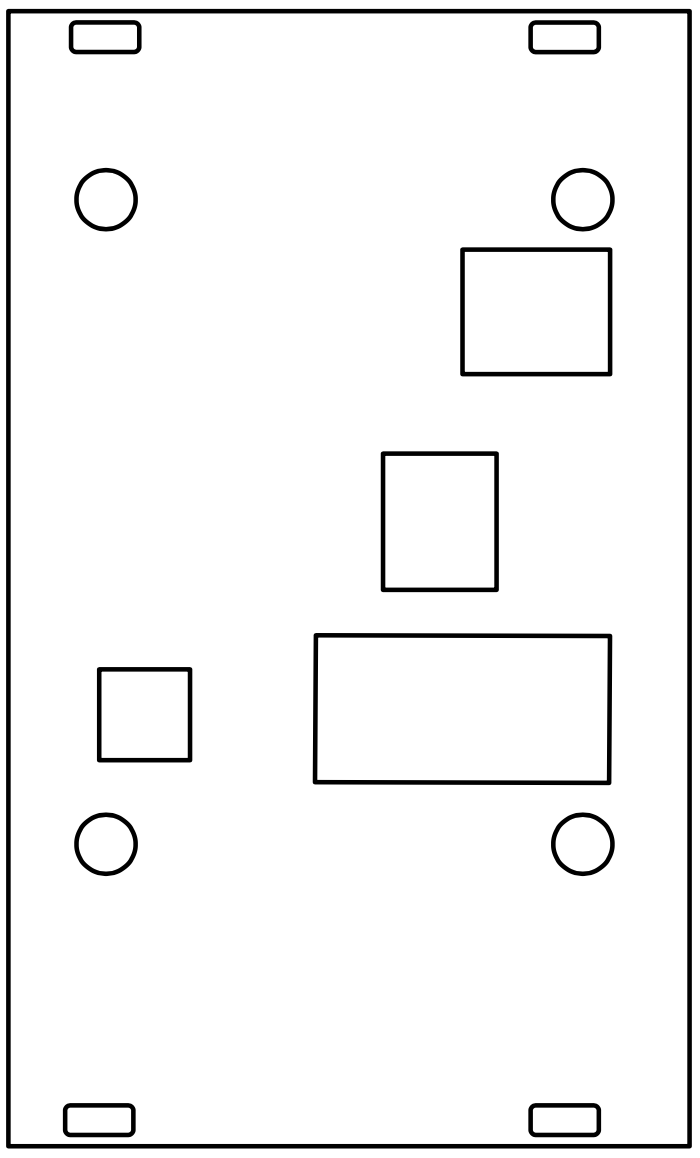
\includegraphics[width=8cm]{images/pcb_acrylic.png}
    \centering
    \caption{Custom cut acrylic design for the PCB}
    \label{acryl}
    \end{figure} 

The challenge with laser cutting the acrylic was to get the precise measurements of everything involved in the design so the acrylic cover fit the Eurorack case and the PCB just right. As shown in Fig. \ref{acryl}, the acrylic has four box-like holes on the four corners to accommodate for the attachment to the Eurorack case. Additionally, the inner four circular holes were for the PCB holes to go through with a screw and nut. The boxes were cut to allow the interactive components of the PCB to be accessible during Demo Day. 

On Demo Day, visitors to our booth could play the piano and hear either the sawtooth wave or the triangle wave output of the VCO--their choice! They could fiddle with the rotary encoder or type integer values into the desktop GUI to change the sound of the music. They could save particular sounds, and then load any previously saved sound onto the synth in an instant. We had a great time demoing our project for all of our visitors. 

\section{Conclusion}

This synthesizer essentially fulfills the goals outlined in our project proposal; we generated an analog signal to produce music, and we preserved the convenience of a digital synth by allowing users to save and load their favorite sounds. Though we weren't able to include as many modules as we would have liked, we are satisfied with the integration of our basic components and we are proud of our synth. We created a unique and scalable product that caters to a niche audience within the world of music production.

\section{Acknowledgements}
We appreciate Professor Brunvand and Professor Stevens for helping us nuture this idea and bring our project to fruition. We thank Dr. Rasmussen for pointing us in the right direction for debugging analog circuits. Dirk Lamb was Michelle's team partner for the Embedded Systems Design final project, for which they built the digipot and rotary encoder circuitry and the embedded code to go with it. Dirk Lamb also showed the team how to use Ableton Live, and for that we thank him \cite{dirk}! 

\addtolength{\textheight}{-12cm}  

%%%%%%%%%%%%%%%%%%%%%%%%%%%%%%%%%%%%%%%%%%%%%%%%%%%%%%%%%%%%%%%%%%%%%%%%%%%%%%%%


\begin{thebibliography}{99}

\bibitem{MAKE} R. Wilson, Make: analog synthesizers. Sebastopol, CA: Maker Media, 2014.
\bibitem{VCO} \textit{SIMPLE 1v/oct OSCILLATOR}, S. Battle, Accessed on: Sept. 26, 2019. [Online] Available: https://www.lookmumnocomputer.com/projects/\#/cem-3340-diy-simple
\bibitem{VCF} \textit{LM13700 Dual Operational Transconductance Amplifiers With Linearizing Diodes and Buffers}, Texas Instruments, Nov. 2015
\bibitem{pot} \textit{Quad Channel, 128-/256-Position, I2C/SPI, Nonvolatile Digital Potentiometer}, Norwood, MA: Analog Devices, 2019
\bibitem{rotenc} \textit{PEC12R - 12 mm Incremental Encoder}, Bourns Pro Audio
\bibitem{filechooser} \textit{FileChooser}, Accessed on: Nov. 5, 2019. [Online] Available: https://kivy.org/doc/stable/api-kivy.uix.filechooser.html
\bibitem{dirk} Dirk Lamb, dirk.lamb31@gmail.com
\bibitem{pyserial} \textit{Short introduction}, Accessed on: Oct. 28, 2019. [Online] Available: https://pyserial.readthedocs.io/en/latest/shortintro.html


\end{thebibliography}

\end{document}
